\section{Random coefficients estimation and a comparison of the three models}\label{sec:C-rc-est}

Sections \ref{sec:C-vertical} and \ref{sec:C-logit-est} estimated two misspecified models on the simulated market of
\cref{sec:C-simulate}. The vertical model allowed one dimension of taste, and the logit allowed none beyond the
idiosyncratic shock. In this problem we estimate the model that generated the data. We take the dispersion of tastes
$\Sigma$ as known. This isolates the two steps on which random coefficients estimation rests. The first is the
inversion of market shares by the contraction of \citet{BerryLevinsohnPakes1995}. The second is linear instrumental
variables on the recovered mean utilities. With the true structure in hand we then compare the three models on elasticities, diversion, markups,
recovered costs and the predicted effects of a merger. \Cref{sec:08-worked} estimates $\Sigma$ itself on the same data.

\subsection{Statement}

Use the data of \cref{sec:C-simulate} and \cref{ass:C-est}. In each of the 100 markets the econometrician observes
prices, realized shares $s^{obs}_{jt}$, characteristics $x_{jt}$, the milk price $w_{jt}$, the owners and the market
size. The realized shares are the shares $\hat s_{jt}$ of \eqref{eq:C-realized}. Demand is the random coefficients logit
\eqref{eq:C-rc-utility},
\begin{equation}\label{eq:C-rc-model}
  u_{ijt} = \delta_{jt} + \mu_{ijt} + \epsilon_{ijt}, \qquad \mu_{ijt} = \tilde x_{jt}\Sigma\nu_i, \qquad
  \delta_{jt} = x_{jt}\beta - \alpha p_{jt} + \xi_{jt},
\end{equation}
with $\tilde x_{jt} = (x_{jt}, p_{jt})$, $\nu_i \sim N(0, I_4)$, independent type-I extreme value shocks
$\epsilon_{ijt}$, and $u_{i0t} = \epsilon_{i0t}$. The term $\mu_{ijt}$ is the consumer-specific deviation from the mean
utility $\delta_{jt}$. The scale matrix $\Sigma = \diag(0.5, 0.2, 0.3, 0.5)$ is known, with $\Sigma_{pp} = 0.5$ its
price entry. The linear parameters $\theta_1 = (\beta, \alpha)$ are unknown. Firms A to D own the products listed in
\cref{tab:C-products} and set prices in a multi-product Bertrand-Nash equilibrium.

\begin{enumerate}[label=(\alph*)]
  \item Draw $n_s = 1{,}000$ vectors $\nu_{it}$ for each market and keep them fixed for the rest of the problem. Why
  must the draws stay fixed?
  \item Write the simulated share function $s_t(\delta_t, \Sigma)$ for a given $\Sigma$ and derive its derivatives
  with respect to $\delta_t$.
  \item Starting from the logit inversion, recover $\delta_t$ in every market with the iteration
  $\delta^{(h+1)}_t = \delta^{(h)}_t + \ln s^{obs}_t - \ln s_t(\delta^{(h)}_t, \Sigma)$. Prove that it converges. Report
  $\delta_t$ for market 0, explain why every mean utility falls relative to the logit start, and account for the gaps
  between the recovered and the true mean utilities.
  \item Estimate $(\beta, \alpha)$ from the recovered mean utilities. Give the identification argument and standard
  errors.
  \item Compute the elasticity matrix of market 0 with the estimation draws, including the outside good. Compare it
  with the true matrix and with the vertical and logit matrices of Sections \ref{sec:C-vertical} and
  \ref{sec:C-logit-est}. Compute the diversion from each product to the outside good. Recover marginal costs under the
  estimated model and compare the three models.
  \item Firms B and C merge. Predict the new equilibrium of market 0 with the logit, the estimated random coefficients
  model and the true model.
  \item How would you proceed if $\Sigma$ were unknown?
\end{enumerate}

\subsection{Solution}

\casehead{Part (a)}
For each market $t$ we draw $n_s = 1{,}000$ vectors $\nu_{it} \sim N(0, I_4)$, $i = 1, \dots, n_s$, once and store
them. The draws use their own seed (2030), different from the seed of the firms' 100 draws in \cref{sec:C-simulate}.
The econometrician does not know which consumer types the firms had in mind. Draws are independent across
markets. The draws stay fixed for three reasons.
\begin{enumerate}
  \item With fixed draws, the simulated share function of part (b) is a deterministic and smooth function of
  $\delta_t$, and the iteration of part (c) has a well-defined fixed point. With fresh draws at every step, the map
  itself would change from one iteration to the next. The iterates would then wander around the solution by the size
  of the simulation error, which part (c) puts at a few hundredths. A stopping rule with tolerance $10^{-10}$ would
  never be met.
  \item When $\Sigma$ is estimated (part (g)), the GMM objective must be a deterministic function of $\Sigma$.
  Otherwise the optimizer compares objective values computed with different draws, and its minimizer is not defined.
  With fixed draws the objective is a smooth function of $\Sigma$, and the simulation asymptotics of
  \citet{PakesPollard1989} can be applied. Because the simulated shares enter the moments through the nonlinear
  inversion, simulation error also adds a bias of order $\frac{1}{n_s}$ (\cref{prop:08-simbias}). Consistency
  therefore requires the number of draws to grow with the sample. With many draws, the simulation error adds a term
  to the variance \citep{BerryLevinsohnPakes1995}.
  \item Fixed draws make the estimator a function of the data and the draws. Its simulation error can then be measured
  by solving again with other draws, as we do in part (c).
\end{enumerate}

\casehead{Part (b)}
Given the draws and a candidate vector of mean utilities $\delta_t = (\delta_{jt})_{j \in \mathcal{J}_t}$, the
individual choice probabilities are
\begin{equation}\label{eq:C-rc-sij-delta}
  s_{ijt}(\delta_t) = \frac{e^{\delta_{jt} + \mu_{ijt}}}{1 + \sum_{k \in \mathcal{J}_t}e^{\delta_{kt} + \mu_{ikt}}} ,
  \qquad
  s_{i0t}(\delta_t) = \frac{1}{1 + \sum_{k \in \mathcal{J}_t}e^{\delta_{kt} + \mu_{ikt}}} ,
\end{equation}
with $\mu_{ijt} = \tilde x_{jt}\Sigma\nu_{it}$, and the simulated shares are
\begin{equation}\label{eq:C-rc-sdelta}
  s_{jt}(\delta_t, \Sigma) = \frac{1}{n_s}\sum_{i=1}^{n_s}s_{ijt}(\delta_t) .
\end{equation}
This is the simulator \eqref{eq:C-rc-simshare} with $\delta_t$ as its argument. Prices enter only through
$\mu_{ijt}$, and they stay at their observed values throughout the inversion. We evaluate \eqref{eq:C-rc-sij-delta}
with the overflow-safe rule of \cref{sec:C-simulate}, part (b). The convergence argument of part (c) rests on the
derivatives of this function.

\begin{lemma}[Derivatives of the simulated shares]\label{lem:C-sdelta}
For every market and every $\delta_t$:
\begin{enumerate}[label=(\roman*)]
  \item $\frac{\partial s_{jt}}{\partial\delta_{kt}} = \frac{1}{n_s}\sum_{i=1}^{n_s}s_{ijt}\big(\indic\{j = k\} -
  s_{ikt}\big)$.
  \item $0 < \frac{\partial s_{jt}}{\partial\delta_{jt}} < s_{jt}$, and $\frac{\partial s_{jt}}{\partial\delta_{kt}} <
  0$ for $k \ne j$.
  \item $\sum_{k \in \mathcal{J}_t}\frac{\partial s_{jt}}{\partial\delta_{kt}} = \frac{1}{n_s}\sum_{i=1}^{n_s}s_{ijt}
  s_{i0t} > 0$.
\end{enumerate}
\end{lemma}

\begin{proof}
Fix a draw, drop $t$, and write $V_{ik} = \delta_k + \mu_{ik}$ and $E_i = 1 + \sum_k e^{V_{ik}}$. By the quotient rule,
\[
  \frac{\partial s_{ij}}{\partial V_{ik}}
  = \frac{\indic\{j = k\}e^{V_{ij}}E_i - e^{V_{ij}}e^{V_{ik}}}{E_i^2}
  = s_{ij}\big(\indic\{j = k\} - s_{ik}\big) .
\]
Since $\frac{\partial V_{ik}}{\partial\delta_k} = 1$, averaging over draws gives (i). For (ii), $0 < s_{ij} < 1$
implies $0 < s_{ij}(1 - s_{ij}) < s_{ij}$ and $-s_{ij}s_{ik} < 0$. For (iii),
$\sum_k s_{ij}(\indic\{j = k\} - s_{ik}) = s_{ij}(1 - \sum_k s_{ik}) = s_{ij}s_{i0}$.
\end{proof}

\casehead{Part (c)}
For market $t$ define the map
\begin{equation}\label{eq:C-blp-map}
  f_t(\delta_t) = \delta_t + \ln s^{obs}_t - \ln s_t(\delta_t, \Sigma) ,
\end{equation}
with logarithms taken element by element. A vector $\delta_t$ is a fixed point of $f_t$ if and only if
$s_t(\delta_t, \Sigma) = s^{obs}_t$, so the fixed points are exactly the mean utilities that rationalize the observed
shares. The iteration $\delta^{(h+1)}_t = f_t(\delta^{(h)}_t)$ is the contraction of
\citet[eq.~6.8]{BerryLevinsohnPakes1995}, written as eq.~(12) of \citet[p.~533]{Nevo2000a}. Each step raises
$\delta_{jt}$ when the model under-predicts the share of product $j$ and lowers it otherwise.

\begin{proposition}[Convergence of the share inversion]\label{prop:C-blp-contraction}
For every market $t$ and every $\delta_t$,
\begin{equation}\label{eq:C-blp-derivs}
  \frac{\partial f_{jt}}{\partial\delta_{kt}} \ge 0 \ \text{ for all } j, k , \qquad
  \eta_{jt}(\delta_t) \equiv \sum_{k \in \mathcal{J}_t}\frac{\partial f_{jt}}{\partial\delta_{kt}}
  = 1 - \frac{\sum_i s_{ijt}s_{i0t}}{\sum_i s_{ijt}} < 1 .
\end{equation}
The equation $s_t(\delta_t, \Sigma) = s^{obs}_t$ therefore has exactly one solution $\delta^*_t$, and the iteration
converges to it from any starting value. If $\eta_{jt} \le \bar\eta < 1$ for every $j$ on a convex set that
contains $\delta^*_t$ and the iterates, then for every $h \ge 0$
\begin{equation}\label{eq:C-blp-rate}
  \big\|\delta^{(h)}_t - \delta^*_t\big\|_\infty \le \bar\eta^{h}\big\|\delta^{(0)}_t - \delta^*_t\big\|_\infty ,
  \qquad
  \big\|\delta^{(h+1)}_t - \delta^{(h)}_t\big\|_\infty \le \bar\eta^{h}\big\|\delta^{(1)}_t - \delta^{(0)}_t\big\|_\infty .
\end{equation}
\end{proposition}

\begin{proof}
Take $F$ in \cref{cor:08-rowsum} to be the distribution that puts mass $\frac{1}{n_s}$ on each draw, so that its
integrals are the averages of \cref{lem:C-sdelta}. The corollary then gives \eqref{eq:C-blp-derivs}, which is
condition (1) of \cref{thm:08-contraction}. This $F$ has finite support,
so the integrability condition of \cref{thm:08-berry94} holds. That theorem then gives the unique solution
$\delta^*_t$.

For the rate, drop $t$, fix $j$ and apply the mean value theorem on the segment between $\delta^*$ and $\delta$:
\[
  f_j(\delta) - f_j(\delta^*) = \sum_k\frac{\partial f_j}{\partial\delta_k}(\tilde\delta)\,(\delta_k - \delta^*_k)
\]
for some $\tilde\delta$ on the segment. The derivatives are nonnegative and sum to at most $\bar\eta$, so
$|f_j(\delta) - \delta^*_j| \le \bar\eta\|\delta - \delta^*\|_\infty$, using $f_j(\delta^*) = \delta^*_j$. Taking the
maximum over $j$ and iterating gives the first inequality in \eqref{eq:C-blp-rate}. The second follows in the same way
from $\delta^{(h+1)} - \delta^{(h)} = f(\delta^{(h)}) - f(\delta^{(h-1)})$.

\Cref{thm:08-berry94} proves convergence for a truncated iteration. The untruncated iteration also converges from any
start. Let $B$ be the sup-norm ball of radius $\|\delta^{(0)} - \delta^*\|_\infty$ around $\delta^*$. It is convex and
compact. The row sums are continuous and below one, so their maximum $\bar\eta$ on $B$ is below one. The bound
$|f_j(\delta) - \delta^*_j| \le \bar\eta\|\delta - \delta^*\|_\infty$ then holds on $B$, so every iterate stays in $B$.
Hence \eqref{eq:C-blp-rate} applies.
\end{proof}

The row sum has a simple meaning. By Bayes' rule over the draws, as in \cref{prop:C-buyer-alpha},
$\frac{\sum_is_{ijt}s_{i0t}}{\sum_is_{ijt}}$ is the probability that a buyer of product $j$ would choose the outside
good in a new choice situation. So $\eta_{jt}$ is one minus the outside-good probability of $j$'s buyers. The
iteration converges fast when the buyers of every product often choose the outside good, which happens when the outside
share is large. It slows down when inside goods dominate the market (\cref{sec:08-inversion}).

We start from the logit inversion $\delta^{(0)}_{jt} = \ln s^{obs}_{jt} - \ln s^{obs}_{0t}$. It is the exact solution
when $\Sigma = 0$, because then every $s_{ijt}$ is the logit probability at $\delta_t$. We stop when
$\|\delta^{(h+1)}_t - \delta^{(h)}_t\|_\infty < 10^{-10}$. The iteration converges in every market, in 11 to 18
iterations (13.9 on average). At the solution the largest gap between log simulated and log observed shares is
$2.5\times10^{-11}$.

Market 0 shows the proposition at work. At the solution the row sums lie between 0.207 and 0.234. The buyers of each
product choose the outside good with probability 0.766 to 0.793, against 0.855 for all simulated consumers. The largest
row sum along the path of the iteration is $\bar\eta = 0.261$. The first step has size 0.280, so by the second
inequality in \eqref{eq:C-blp-rate} the stopping rule must be met by iteration 18. It is met at iteration 15. After the
first step, the ratio of successive step sizes settles at 0.216. This ratio estimates the largest eigenvalue of the
Jacobian of $f_0$ at the solution, which cannot exceed the largest row sum because the Jacobian has nonnegative
entries. Over all 100 markets the largest row sum at the solution is 0.295.

\Cref{tab:C-delta0} reports the mean utilities of market 0. The recovered values are close to the true ones,
$x_{j}\beta - \alpha p_{j0} + \xi_{j0}$, and every one of them lies below its logit start. The next proposition
explains the second fact.

\begin{table}[htbp]
\centering
\caption{Mean utilities in market 0 with $\Sigma$ known}
\label{tab:C-delta0}
\footnotesize
\setlength{\tabcolsep}{4.5pt}
\begin{tabular}{@{}lccccccccc@{}}
\toprule
 & & & Logit start & \multicolumn{2}{c}{Recovered $\hat\delta_j$} & True & \multicolumn{2}{c}{Gap from truth} & S.e.\ of \\
\cmidrule(lr){5-6}\cmidrule(lr){8-9}
Product & Firm & Buyers $q_j$ & $\delta^{(0)}_j$ & 1,000 draws & 100,000 draws & $\delta_j$ & Simulation & Sampling &
$\ln\hat s_j$ \\
\midrule
2 & C & 51 & $-5.110$ & $-5.405$ & $-5.411$ & $-5.581$ & 0.007 & 0.170 & 0.140 \\
3 & C & 249 & $-3.524$ & $-3.666$ & $-3.701$ & $-3.675$ & 0.035 & $-0.026$ & 0.063 \\
4 & B & 124 & $-4.221$ & $-4.547$ & $-4.551$ & $-4.657$ & 0.005 & 0.105 & 0.089 \\
6 & B & 201 & $-3.738$ & $-3.868$ & $-3.905$ & $-3.962$ & 0.037 & 0.058 & 0.070 \\
8 & A & 553 & $-2.726$ & $-2.903$ & $-2.935$ & $-2.941$ & 0.032 & 0.006 & 0.041 \\
9 & D & 57 & $-4.998$ & $-5.324$ & $-5.330$ & $-5.193$ & 0.006 & $-0.137$ & 0.132 \\
10 & C & 199 & $-3.748$ & $-3.874$ & $-3.910$ & $-3.843$ & 0.036 & $-0.067$ & 0.070 \\
\bottomrule
\end{tabular}

\vspace{3pt}
\begin{minipage}{0.97\textwidth}
\footnotesize Notes: $M_0 = 9{,}880$ consumers, outside share 0.8549. The logit start is
$\ln s^{obs}_j - \ln s^{obs}_0$. The recovered values solve $s_t(\delta_t, \Sigma) = s^{obs}_t$ for $t = 0$
with the 1,000 estimation draws (seed 2030) and with 100,000 draws (seed 2032). The simulation gap is the difference between the two
solutions, and the sampling gap is the 100,000-draw solution minus the true value. The last column is
$\sqrt{\frac{1 - s_j}{q_j}}$ from \eqref{eq:C-logshare-var}. Computed with \texttt{figures/appC/src/appC\_rc.py}.
\end{minipage}
\end{table}

\begin{proposition}[Mean utilities below the logit inversion]\label{prop:C-delta-lower}
\begin{enumerate}[label=(\roman*)]
  \item Suppose a market has one inside product with observed share $s^{obs} < \frac{1}{2}$, and the random term
  $\mu_i$ has a nondegenerate distribution that is symmetric about zero. Let $\mathcal{L}(u) = \frac{e^u}{1 + e^u}$ be the logistic distribution function, and let
  $\delta^*$ solve $\E[\mathcal{L}(\delta + \mu_i)] = s^{obs}$. Then
  \[
    \delta^* < \ln\frac{s^{obs}}{1 - s^{obs}} .
  \]
  \item With several inside products, a diagonal $\Sigma$ and $\lVert\Sigma\rVert \to 0$, the gap
  $r_{jt} = \ln\frac{s^{obs}_{jt}}{s^{obs}_{0t}} - \delta^*_{jt}$ is positive up to terms of order $\lVert\Sigma\rVert^3$
  whenever $\|\tilde x_{jt}\Sigma\| > 2\|\bar x_t\Sigma\|$, where $\bar x_t = \sum_k s_{kt}\tilde x_{kt}$ and
  $\|\cdot\|$ is the Euclidean norm.
\end{enumerate}
\end{proposition}

\begin{proof}
(i) Let $\delta_L = \ln\frac{s^{obs}}{1 - s^{obs}}$, the logit inversion, so that $\mathcal{L}(\delta_L) = s^{obs}$ and
$\delta_L < 0$. For $m \ge 0$ define $g(m) = \mathcal{L}(\delta_L + m) + \mathcal{L}(\delta_L - m) - 2\mathcal{L}(\delta_L)$. Then
$g(0) = 0$ and
\[
  g'(m) = \ell(\delta_L + m) - \ell(\delta_L - m) ,
\]
where $\ell(u) = \mathcal{L}(u)(1 - \mathcal{L}(u))$ is the logistic density. It is symmetric about zero and strictly
decreasing in $|u|$. For $m > 0$, $\delta_L < 0$ gives $|\delta_L + m| < |\delta_L| + m = |\delta_L - m|$, so
$g'(m) > 0$ and $g(m) > 0$. By the symmetry of $\mu_i$,
\[
  \E[\mathcal{L}(\delta_L + \mu_i)] = \frac{1}{2}\E\big[\mathcal{L}(\delta_L + \mu_i) + \mathcal{L}(\delta_L - \mu_i)\big]
  = \mathcal{L}(\delta_L) + \frac{1}{2}\E\big[g(|\mu_i|)\big] > s^{obs} ,
\]
with strict inequality because $\mu_i \ne 0$ with positive probability. The function
$\delta \mapsto \E[\mathcal{L}(\delta + \mu_i)]$ is strictly increasing, so its solution $\delta^*$ lies below $\delta_L$.

(ii) By \cref{prop:C-gap-approx}, with $a = \tilde x_{jt}\Sigma$ and $b = \bar x_t\Sigma$ (row vectors, $\Sigma$ diagonal),
$r_{jt} = \frac{1}{2}\|a\|^2 - a b^\top + O(\lVert\Sigma\rVert^3)$. The Cauchy-Schwarz inequality gives $ab^\top \le \|a\|\,\|b\|$,
so $r_{jt} \ge \|a\|\big(\frac{1}{2}\|a\| - \|b\|\big) + O(\lVert\Sigma\rVert^3)$, which is positive when $\|a\| > 2\|b\|$.
\end{proof}

Part (i) is the convexity argument in its cleanest form. The logit probability is convex below one half, so spreading
utility symmetrically around $\delta$ raises the average choice probability. To match the observed share, the mean
utility must fall. Part (ii) covers our design. The vector $\bar x_t$ averages the inside products with weights equal to
their shares, which sum to the inside share of at most 0.21. So $\|\bar x_t\Sigma\|$ is a small fraction of
$\max_k\|\tilde x_{kt}\Sigma\|$, and the condition holds unless products are very different. In the data every one of
the 654 recovered mean utilities lies below its logit start. The gap $r_{jt}$, studied in \cref{sec:C-logit-est},
part (e), has mean 0.247 (\cref{fig:C-gap}). In market 0 it is smallest for product 10, the cheapest, and largest for
products 4 and 9, which are expensive and organic and therefore have the largest $\|\tilde x_{jt}\Sigma\|$.

The gaps from the truth have two sources, which we separate by solving the inversion again with 100,000 draws:
\begin{equation}\label{eq:C-delta-gap}
  \hat\delta_{jt} - \delta_{jt} = \big(\hat\delta_{jt} - \hat\delta^{100k}_{jt}\big) + \big(\hat\delta^{100k}_{jt} -
  \delta_{jt}\big) .
\end{equation}
The first term is simulation error from using 1,000 draws. In market 0 it lies between 0.005 and 0.037. It has the same
sign for every product, which reflects the draws that all products share. It is of the same order as the relative
simulation standard error of the shares, the standard deviation of $s_{ij0}$ across draws divided by
$\sqrt{n_s}\,s_{j0}$, which lies between 0.020 and 0.030. The second term is sampling error. Realized shares are
proportions among about 10,000 consumers, and by \eqref{eq:C-logshare-var} the log share of product $j$ has standard
error near $\sqrt{\frac{1 - s_{j}}{q_{j}}}$. Products 2, 4 and 9 miss the truth by 1.0 to 1.2 of these standard errors,
and the others by less. Both errors are independent across markets. To first order they have mean zero and are uncorrelated with the
instruments, so they act as extra noise in the regression of part (d). The log transformation adds a small
second-order bias that depends on the share, of order $\frac{1}{q_j}$.

\casehead{Part (d)}
With $\Sigma$ known, the recovered mean utilities satisfy the linear equation
\begin{equation}\label{eq:C-rc-linear}
  \hat\delta_{jt} = x_{jt}\beta - \alpha p_{jt} + \xi_{jt} + e_{jt} ,
\end{equation}
where $e_{jt} = \hat\delta_{jt} - \delta_{jt}$ collects the simulation and sampling errors of part (c). Price is
correlated with $\xi_{jt}$ because firms observe $\xi_{jt}$ when they set prices (\cref{sec:C-logit-est}, part (a)).
We therefore estimate \eqref{eq:C-rc-linear} by 2SLS with the instruments of \eqref{eq:C-logit-moments}: the milk price
and the six sums of characteristics and counts of the firm's other products and of rival products. The parameters are
identified by the moment conditions $\E[z_{jt}^\top(\xi_{jt} + e_{jt})] = 0$ and the rank condition of
\cref{sec:C-logit-est}. The error $e_{jt}$ comes from consumers' choices and from the econometrician's draws, given
prices. To first order it has mean zero conditional on $z_{jt}$, so it adds noise without adding bias. The
regressors and instruments are those of the logit, so the first stage is the one in \cref{tab:C-firststage}.

\begin{table}[htbp]
\centering
\caption{Demand estimates with $\Sigma$ known}
\label{tab:C-rc-demand}
\footnotesize
\setlength{\tabcolsep}{4pt}
\begin{tabular}{@{}lccccc@{}}
\toprule
 & Logit & \multicolumn{3}{c}{Random coefficients, $\Sigma$ known} & \\
\cmidrule(lr){2-2}\cmidrule(lr){3-5}
 & 2SLS & OLS & 2SLS & \makecell{2SLS, milk\\price only} & True \\
\midrule
Constant & $-1.184$ (0.329) & $-1.355$ (0.227) & $-1.061$ (0.330) & $-1.042$ (0.335) & $-1.00$ \\
Sugar content & 0.190 (0.158) & 0.088 (0.122) & 0.168 (0.158) & 0.173 (0.156) & 0.20 \\
Organic & 0.153 (0.141) & $-0.002$ (0.097) & 0.114 (0.142) & 0.121 (0.143) & 0.15 \\
Price coefficient $\alpha$ & 2.641 (0.412) & 2.573 (0.252) & 2.926 (0.413) & 2.948 (0.415) & 3.00 \\
\midrule
First-stage $F$ & 92.5 & & 92.5 & & \\
Hansen $J$ (df, $p$) & 8.82 (6, 0.18) & & 8.16 (6, 0.23) & & \\
Observations & 654 & 654 & 654 & 654 & \\
\bottomrule
\end{tabular}

\vspace{3pt}
\begin{minipage}{0.97\textwidth}
\footnotesize Notes: The dependent variable is $\ln s^{obs}_{jt} - \ln s^{obs}_{0t}$ for the logit and the recovered
$\hat\delta_{jt}$ otherwise. Standard errors in parentheses are clustered by market with the factor
$\frac{G}{G - 1}\frac{N - 1}{N - K}$ and condition on $\Sigma$. The first and third 2SLS columns use the milk price and
the six competition instruments, and the last uses the milk price alone. The logit column repeats \cref{tab:C-logit-demand}. Computed with
\texttt{figures/appC/src/appC\_rc.py}.
\end{minipage}
\end{table}

\Cref{tab:C-rc-demand} reports the estimates. The 2SLS estimate of the price coefficient is 2.926, within 0.18
standard errors of the true value of 3. OLS gives 2.573, biased toward zero for the same reason as in the logit. Using
the milk price alone gives 2.948 with a slightly larger standard error, so the six competition instruments add little,
as in \cref{sec:C-logit-est}. Hansen's test does not reject the overidentifying restrictions ($J = 8.16$, $p = 0.23$).
The coefficients on sugar and organic production are close to the truth but imprecise. They are identified from ten
products whose characteristics never change, so the data contain only ten distinct combinations of characteristics.

The comparison with the logit is exact. By \cref{prop:C-logit-bias}, the logit estimate equals the random coefficients
estimate minus the 2SLS price coefficient of the gap term $r_{jt}$ on the same regressors and instruments. That
coefficient is 0.284, and the identity $2.641 = 2.926 - 0.284$ holds to machine precision (\cref{sec:C-logit-est},
part (e)). Allowing for the random coefficients
moves the estimate from 0.359 below the truth to 0.074 below it. The remaining gap is well within sampling error. The
estimates also imply sensible individual tastes. Across the 100,000 estimation draws, the smallest price sensitivity
$\alpha_i = \hat\alpha - \Sigma_{pp}\nu_{i4}$ is 0.814, so every simulated consumer dislikes higher prices, as
\cref{prop:C-ms} requires.

The standard errors cluster by market, with the sandwich \eqref{eq:C-clustervar}. The recovered $\hat\delta_t$ depends
only on the shares and draws of market $t$, so the errors are independent across markets and clustering is valid. The
standard errors condition on $\Sigma$. If $\Sigma$ were estimated, $\hat\theta_1 = \hat\theta_1(\hat\Sigma)$ would inherit
the uncertainty in $\hat\Sigma$, and all parameters would be estimated jointly as in part (g).

\casehead{Part (e)}
A change in $p_{kt}$ moves both the mean utility, through $-\alpha$, and the random term, through $\Sigma_{pp}\nu_{i4}$.
For draw $i$ the price coefficient is therefore $-\alpha_i$ with $\alpha_i = \hat\alpha - \Sigma_{pp}\nu_{i4}$. Applying
\cref{lem:C-sdelta}(i) draw by draw, with $\frac{\partial V_{ikt}}{\partial p_{kt}} = -\alpha_i$, gives the share
derivatives
\begin{equation}\label{eq:C-rc-elast}
  \frac{\partial s_{jt}}{\partial p_{kt}} = \frac{1}{n_s}\sum_{i=1}^{n_s}\alpha_is_{ijt}\big(s_{ikt} - \indic\{j = k\}\big) ,
  \qquad
  \frac{\partial s_{0t}}{\partial p_{kt}} = \frac{1}{n_s}\sum_{i=1}^{n_s}\alpha_is_{i0t}s_{ikt} .
\end{equation}
The second formula follows from $\frac{\partial s_{i0t}}{\partial V_{ikt}} = -s_{i0t}s_{ikt}$. The elasticities are
$\varepsilon_{jk} = \frac{\partial s_j}{\partial p_k}\frac{p_k}{s_j}$ and
$\varepsilon_{0k} = \frac{\partial s_0}{\partial p_k}\frac{p_k}{s_0}$. Own entries are negative, so the positive own
elasticity of the book's notation is $-\varepsilon_{jj}$. The estimated matrix uses $\hat\alpha = 2.926$, the recovered
$\hat\delta_0$ and the 1,000 estimation draws. The true matrix uses the true parameters, the true mean utilities and
the firms' 100 draws, the demand system that generated the prices. \Cref{tab:C-rcelast} reports both.

\begin{table}[htbp]
\centering
\caption{Random coefficients elasticities in market 0}
\label{tab:C-rcelast}
\footnotesize
\begin{tabular}{@{}lrrrrrrr@{}}
\toprule
 & \multicolumn{7}{c}{Price of product} \\
\cmidrule(lr){2-8}
Share of & 2 & 3 & 4 & 6 & 8 & 9 & 10 \\
\midrule
\multicolumn{8}{@{}l}{\emph{Panel A. Estimated model ($\hat\alpha = 2.926$, $\Sigma$ known)}} \\
Product 2 & $-3.45$ & 0.10 & 0.08 & 0.07 & 0.24 & 0.04 & 0.07 \\
Product 3 & 0.03 & $-2.68$ & 0.07 & 0.07 & 0.23 & 0.03 & 0.07 \\
Product 4 & 0.03 & 0.10 & $-3.63$ & 0.08 & 0.24 & 0.04 & 0.07 \\
Product 6 & 0.02 & 0.09 & 0.07 & $-2.65$ & 0.23 & 0.03 & 0.07 \\
Product 8 & 0.03 & 0.09 & 0.07 & 0.07 & $-2.79$ & 0.03 & 0.07 \\
Product 9 & 0.03 & 0.10 & 0.08 & 0.08 & 0.24 & $-3.74$ & 0.07 \\
Product 10 & 0.02 & 0.09 & 0.07 & 0.07 & 0.23 & 0.03 & $-2.51$ \\
Outside good & 0.02 & 0.07 & 0.04 & 0.05 & 0.16 & 0.02 & 0.05 \\
\midrule
\multicolumn{8}{@{}l}{\emph{Panel B. True model}} \\
Product 2 & $-3.57$ & 0.12 & 0.09 & 0.08 & 0.29 & 0.05 & 0.09 \\
Product 3 & 0.03 & $-2.74$ & 0.07 & 0.08 & 0.26 & 0.04 & 0.08 \\
Product 4 & 0.03 & 0.12 & $-3.74$ & 0.08 & 0.29 & 0.05 & 0.09 \\
Product 6 & 0.03 & 0.10 & 0.07 & $-2.71$ & 0.25 & 0.04 & 0.08 \\
Product 8 & 0.03 & 0.11 & 0.08 & 0.08 & $-2.84$ & 0.05 & 0.08 \\
Product 9 & 0.03 & 0.12 & 0.09 & 0.08 & 0.29 & $-3.85$ & 0.09 \\
Product 10 & 0.03 & 0.10 & 0.07 & 0.07 & 0.26 & 0.04 & $-2.57$ \\
Outside good & 0.02 & 0.07 & 0.04 & 0.05 & 0.17 & 0.03 & 0.06 \\
\bottomrule
\end{tabular}

\vspace{3pt}
\begin{minipage}{0.97\textwidth}
\footnotesize Notes: Entry $(j, k)$ is $\varepsilon_{jk} = \frac{\partial s_j}{\partial p_k}\frac{p_k}{s_j}$, the
percentage change in the share of the row alternative after a one percent rise in the price of the column product.
Panel A uses the 1,000 estimation draws and the recovered mean utilities. Panel B uses the true parameters and mean
utilities and the firms' 100 draws. Computed with \texttt{figures/appC/src/appC\_rc.py}.
\end{minipage}
\end{table}

The estimated matrix is close to the true one. The largest absolute difference between corresponding entries is 0.11.
The estimated own elasticities run from $-2.51$ to $-3.74$, against $-2.57$ to $-3.85$ in the truth. They are slightly
smaller in magnitude because $\hat\alpha$ is slightly below 3. Three features distinguish the random coefficients
matrix from the other two models.

First, cross elasticities differ within a column. In the logit every off-diagonal entry of column $k$ equals
$\hat\alpha^lp_ks_k$ (\cref{tab:C-lelast}). In Panel A the largest ratio between two cross elasticities in the same
column is 1.21, and in the truth it is 1.27. The pattern has an economic logic. A rise in the price of product 4 raises
the shares of products 2 and 9 by more than those of the other products. The same holds for the columns of products 2
and 9. The three products are the organic ones and also the most expensive. Their buyers have high draws of the
organic taste $\nu_{i3}$ or low price sensitivity $\alpha_i$. When they leave one of these products, they look for
another product that suits the same tastes.

Second, the outside good receives less substitution than the logit implies. The diversion ratio from product $k$ to
the outside good (\cref{sec:C-logit-bertrand}, part (e), and \cref{sec:C-vertical}, part (e)) is
\begin{equation}\label{eq:C-div0}
  D_{k0} = \frac{\frac{\partial s_0}{\partial p_k}}{-\frac{\partial s_k}{\partial p_k}}
  = \frac{\sum_i\alpha_is_{ik}s_{i0}}{\sum_i\alpha_is_{ik}(1 - s_{ik})}
  = \sum_i\varpi_{ik}\frac{s_{i0}}{1 - s_{ik}} , \qquad
  \varpi_{ik} = \frac{\alpha_is_{ik}(1 - s_{ik})}{\sum_l\alpha_ls_{lk}(1 - s_{lk})} .
\end{equation}
The second equality uses \eqref{eq:C-rc-elast}. The third writes $D_{k0}$ as a weighted average of the individual logit
diversion ratios $\frac{s_{i0}}{1 - s_{ik}}$, with weights that favour the draws most likely to buy $k$. In the logit
all draws are alike and $D_{k0} = \frac{s_0}{1 - s_k}$, which lies between 85.9 and 90.6 percent in market 0. Under the
estimated random coefficients model it lies between 79.2 and 86.7 percent, and in the truth between 76.2 and 85.1
percent. The buyers of a product are disproportionately consumers with a high draw of the random constant. Their
probability of choosing the outside good is 0.77 to 0.79, against 0.855 on average, so they divert less of their
purchases to it. The logit cannot represent this selection. It overstates diversion to the outside good by 5 to 10
percentage points relative to the truth and understates diversion among inside goods, which matters for the merger of part (f).

Third, the vertical model is far from both (\cref{tab:C-velast}). Its own elasticities range from $-16.8$ to
$-358.4$. Their mean absolute value, 126.6, is 41 times that of the logit. Each row has at most two nonzero cross elasticities, one for each
neighbour on the price ladder. Only the cheapest product, product 10, loses sales to the outside good, and only 6.4
percent of them. \Cref{fig:C-own-elas} summarizes the own elasticities. \Cref{fig:08-ownelas} shows the logit and random
coefficients panels on the same data.

\begin{figure}[htbp]
\centering
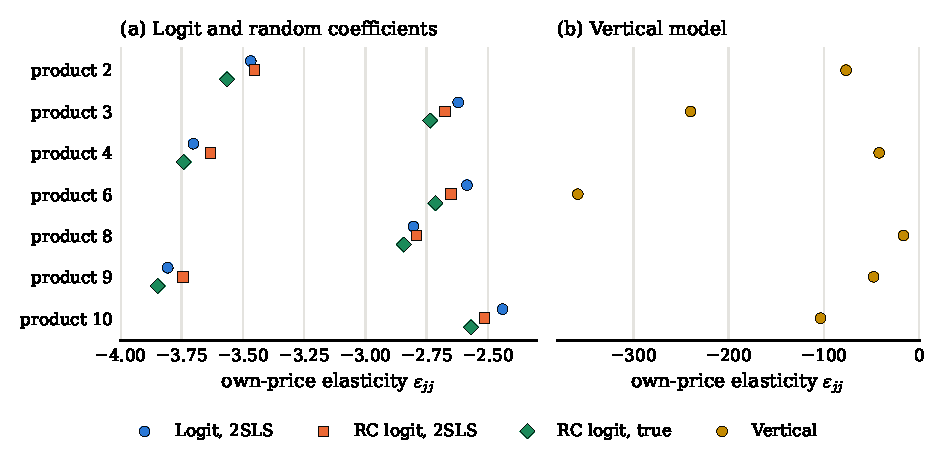
\includegraphics[width=\linewidth]{figures/appC/own_elas.pdf}
\caption{Own-price elasticities in market 0 by product. Panel (a): logit estimated by 2SLS, random coefficients logit
estimated by 2SLS with $\Sigma$ known, and the true random coefficients model. Panel (b): the vertical model, on its own
scale. Computed with \texttt{figures/appC/src/appC\_rc.py}.}
\label{fig:C-own-elas}
\end{figure}

We now recover marginal costs. Under the estimated model, the stacked first-order conditions
\eqref{eq:C-stacked-foc} give
\begin{equation}\label{eq:C-rc-mc-hat}
  \widehat{mc}_t = p_t + \big(\Omega_t \odot \hat\Delta_t^\top\big)^{-1}s^{obs}_t ,
\end{equation}
with $\hat\Delta_t$ the matrix of share derivatives \eqref{eq:C-rc-elast}. We regress $\widehat{mc}_{jt}$ on
$(x_{jt}, w_{jt})$ by OLS. The regressand depends on $\hat\alpha$, so we compute standard errors with a bootstrap over
markets (5,000 resamples, seed 2031) that re-estimates $\hat\alpha$ in each replication. With $\Sigma$ known,
$\hat\delta_t$ does not depend on $\alpha$, so only $\hat\Delta_t$ changes across replications. \Cref{tab:C-compare}
collects the comparison.

\begin{table}[htbp]
\centering
\caption{Three demand models estimated on the same simulated data}
\label{tab:C-compare}
\footnotesize
\setlength{\tabcolsep}{4pt}
\begin{tabular}{@{}lcccc@{}}
\toprule
 & Vertical & Logit & \makecell{Random coefficients\\($\Sigma$ known)} & True \\
\midrule
Price coefficient $\alpha$ & none & 2.641 (0.412) & 2.926 (0.413) & 3.00 \\
Own elasticities, market 0 & $-16.8$ to $-358.4$ & $-2.44$ to $-3.81$ & $-2.51$ to $-3.74$ & $-2.57$ to $-3.85$ \\
Nonzero cross elasticities per row & 1 or 2 & 6 & 6 & 6 \\
Largest ratio within a column & & 1.00 & 1.21 & 1.27 \\
Diversion to outside good, market 0 (\%) & 0 to 6.4 & 85.9 to 90.6 & 79.2 to 86.7 & 76.2 to 85.1 \\
\midrule
Mean markup, all observations & 0.048 & 0.396 & 0.397 & 0.386 \\
Range of markups & 0.000 to 0.515 & 0.379 to 0.426 & 0.368 to 0.452 & 0.348 to 0.451 \\
Correlation with true markups & 0.275 & 0.553 & 0.715 & 1 \\
Mean absolute markup error & 0.340 & 0.014 & 0.013 & 0 \\
\midrule
\multicolumn{5}{@{}l}{\emph{Marginal cost equation}} \\
Constant & 0.674 (0.024) & 0.160 (0.072) & 0.188 (0.060) & 0.20 \\
Sugar content & 0.194 (0.014) & 0.258 (0.010) & 0.246 (0.010) & 0.25 \\
Organic & 0.271 (0.009) & 0.315 (0.006) & 0.305 (0.006) & 0.30 \\
Price of milk & 0.356 (0.031) & 0.532 (0.023) & 0.504 (0.026) & 0.50 \\
\bottomrule
\end{tabular}

\vspace{3pt}
\begin{minipage}{0.97\textwidth}
\footnotesize Notes: All models assume multi-product Bertrand-Nash pricing. Cross elasticities and diversion refer to
market 0. Markup statistics use all 654 observations. Cost equations are OLS regressions of the implied marginal cost
on the characteristics and the milk price. Standard errors are clustered by market for the vertical model, whose markups
contain no estimated parameter. For the logit and the random coefficients model they come from a market bootstrap
that re-estimates $\alpha$ (5,000 replications). Computed with \texttt{figures/appC/src/appC\_rc.py}.
\end{minipage}
\end{table}

The random coefficients model wins on every dimension that depends on substitution. Its cost coefficients are the
closest to the truth, and its implied markups track the true markups across observations more closely (correlation
0.715, against 0.553 for the logit). The mean markups of the logit and the random coefficients model are almost equal.
Both are near $\frac{1}{\hat\alpha}$ corrected for the firm's share, and both overstate the true mean of 0.386 a little
because both price coefficients lie below 3. The vertical model fails on every dimension, for the reasons of
\cref{sec:C-vertical}. Adjacent prices are close, its elasticities explode, and its markups collapse toward zero, so
its cost intercept absorbs the true markup.

\casehead{Part (f)}
Firms B and C merge. In market 0, firm B sells products 4 and 6 and firm C sells products 2, 3 and 10. After the merger
one firm owns all five, while firm A (product 8) and firm D (product 9) are unchanged. We predict the new equilibrium
under three demand models: the logit of \cref{sec:C-logit-est}, the estimated random coefficients model of parts (c) and
(d), and the true model. The procedure is the same for each.
\begin{enumerate}
  \item Recover marginal costs from the pre-merger first-order conditions of the model, \eqref{eq:C-rc-mc-hat} or its
  logit version. For the true model use the true marginal costs. Each model then reproduces the observed prices.
  Solving the pre-merger game again returns them to within $3\times10^{-14}$.
  \item Hold marginal costs, unobserved qualities and draws fixed. As prices move, mean utilities move as
  $\delta_{jt}(p) = \hat\delta_{jt} - \alpha(p_{jt} - p^{obs}_{jt})$, and $\mu_{ijt}$ moves through the price entry of
  $\tilde x_{jt}$.
  \item Replace $\Omega_0$ by the post-merger ownership matrix and solve the first-order conditions. For the logit
  iterate $p \leftarrow mc + \frac{1}{\alpha(1 - S_f(p))}$, using \cref{prop:C-common-markup}. For the random
  coefficients models iterate the Morrow-Skerlos map \eqref{eq:C-ms-zeta}. Each converges in 11 iterations to a tolerance
  of $10^{-12}$, and 20 random starting points lead to the same prices to within $9\times10^{-14}$.
  \item Measure consumer welfare by the log-sum formula (\cref{prop:07-logsum}). A consumer with marginal utility of
  income $\alpha_i$ has expected surplus $\frac{1}{\alpha_i}\ln\big(1 + \sum_je^{V_{ij}}\big)$ up to a constant, and we
  average over draws. The constant cancels from the change.
\end{enumerate}

\begin{table}[htbp]
\centering
\caption{Merger of firms B and C in market 0}
\label{tab:C-merger-m0}
\footnotesize
\setlength{\tabcolsep}{4pt}
\begin{tabular}{@{}lcccccccc@{}}
\toprule
 & & & \multicolumn{3}{c}{Equilibrium price change} & \multicolumn{3}{c}{Upward pricing pressure} \\
\cmidrule(lr){4-6}\cmidrule(lr){7-9}
Product & Firm & Price & Logit & RC est. & RC true & Logit & RC est. & RC true \\
\midrule
2 & C & 1.3200 & 0.0129 & 0.0207 & 0.0220 & 0.0129 & 0.0194 & 0.0204 \\
3 & C & 1.0182 & 0.0129 & 0.0184 & 0.0188 & 0.0132 & 0.0178 & 0.0181 \\
4 & B & 1.4196 & 0.0202 & 0.0309 & 0.0356 & 0.0204 & 0.0296 & 0.0340 \\
6 & B & 0.9993 & 0.0202 & 0.0277 & 0.0305 & 0.0206 & 0.0268 & 0.0294 \\
8 & A & 1.1246 & 0.0001 & 0.0004 & 0.0006 & & & \\
9 & D & 1.4497 & 0.0000 & 0.0002 & 0.0002 & & & \\
10 & C & 0.9429 & 0.0129 & 0.0181 & 0.0185 & 0.0131 & 0.0174 & 0.0177 \\
\midrule
Mean change, merging & & & 0.0158 & 0.0231 & 0.0251 & & & \\
Outside share, before, after & & & \makecell{0.8549\\0.8578} & \makecell{0.8549\\0.8589} &
\makecell{0.8463\\0.8507} & & & \\
Change in consumer surplus & & & $-12.78$ & $-18.37$ & $-20.39$ & & & \\
Change in merged profit & & & 0.28 & 0.58 & 0.72 & & & \\
Change in rivals' profit & & & 0.83 & 1.68 & 2.13 & & & \\
Change in total surplus & & & $-11.67$ & $-16.11$ & $-17.54$ & & & \\
\bottomrule
\end{tabular}

\vspace{3pt}
\begin{minipage}{0.97\textwidth}
\footnotesize Notes: Firm B owns products 4 and 6 and firm C owns products 2, 3 and 10 in market 0. Upward pricing
pressure is $\sum_kD_{jk}(p_k - mc_k)$ over the partner firm's products, evaluated before the merger. Surplus and profit
changes are totals over the $M_0 = 9{,}880$ consumers, in the same money units as prices. The true model's outside
share differs before the merger because it uses expected rather than realized shares. Computed with
\texttt{figures/appC/src/appC\_rc\_merger.py}.
\end{minipage}
\end{table}

\Cref{tab:C-merger-m0} reports the predictions. Under the logit, the price increase is the same for every product of a
merging firm, 0.0129 for firm C and 0.0202 for firm B. \Cref{prop:C-common-markup} explains it. Logit
markups are common within a firm, so after the merger the new firm sets one markup $\frac{1}{\alpha(1 - S_{BC})}$ on
all five products. That markup is 0.4117, up from 0.3988 for firm C and 0.3915 for firm B. Firm B's products start from
the lower markup, so they rise more. Under the random coefficients models the increases differ across products and are
largest for products 4 and 6.

The logit understates the merger's effect. The mean increase on the merging products is 0.0158 under the logit, 0.0231
under the estimated random coefficients model and 0.0251 in the truth. The logit captures 63 percent of the true effect
and the estimated model 92 percent. In percentage terms the true increases range from 1.7 to 3.1 percent. The source is
diversion between the merging firms. Consider the share of a merging product's lost sales that goes to the partner firm.
It is 0.033 to 0.052 under the logit, 0.044 to 0.075 under the estimated model and 0.046 to 0.088 in the truth. The logit sends too
many lost sales to the outside good, as part (e) showed, so it sees the two firms as weaker competitors than they are.

First-order upward pricing pressure, defined in \cref{sec:C-logit-bertrand}, part (g), is the opportunity cost
$\sum_kD_{jk}(p_k - mc_k)$ of sales diverted to the partner \citep{FarrellShapiro2010}, discussed in \cref{sec:11-upp}.
It is close to the equilibrium price change in all three models.
For product 4 in the truth, for example, it is 0.0340 against an equilibrium increase of 0.0356. Inside shares are
small, so pass-through is close to one and the feedback among prices is weak. Rivals raise their prices only slightly,
by at most 0.0006, because prices are strategic complements. Consumer surplus falls by 20.39 in the truth, while the
merged firm gains 0.72 and its rivals 2.13. Without cost savings the merger lowers total surplus. The logit predicts
a loss of 11.67, about two thirds of the true loss of 17.54.

The two estimated models agree here more than they would in many markets. Inside shares are small and the products are
similar, so all predicted increases are below 4 percent. The gap
between the logit and the random coefficients model would widen with larger inside shares or more dispersed tastes. It
would also widen if the merging products were closer in characteristics, as in a merger of the owners of the three
organic products.

We do not solve the merger under the vertical model, because its prediction would depend mainly on the price ladder.
In the vertical model every lost sale goes to a neighbour on the price ladder. In market 0 the ladder runs through
products 10, 6, 3, 8, 2, 4 and 9 in increasing order of price. Both neighbours of product 6 belong to firm C, so all of product 6's lost
sales go to the partner. The share is 0.936 for product 10, 0.879 for product 3, 0.605 for product 2 and 0.488 for
product 4. The merger therefore internalizes much of the competition each merging product faces, while the
pre-merger markups that would enter the upward pricing pressure are near zero. A prediction built on these two
artefacts would tell us about the price gaps in market 0 more than about preferences.

\casehead{Part (g)}
When $\Sigma$ is unknown we estimate $\theta = (\theta_1, \theta_2)$, where $\theta_2$ collects the four diagonal
entries of $\Sigma$. The estimator is GMM with the nested fixed point algorithm of \citet{BerryLevinsohnPakes1995}, as
laid out by \citet[Section 3.3]{Nevo2000a}. The steps are as follows.
\begin{enumerate}
  \item Fix the draws, as in part (a).
  \item Inner loop. For a trial $\theta_2$, solve $s_t(\delta_t, \Sigma) = s^{obs}_t$ in every market by the iteration
  of part (c), starting from the solution at the previous trial value. Use a tight tolerance, because errors in
  $\delta$ pass into the objective and can stop the outer search at false minima \citep{DubeFoxSu2012}.
  \item Form the structural error $\xi_{jt}(\theta) = \delta_{jt}(\theta_2) - x_{jt}\beta + \alpha p_{jt}$
  \citep[eq.~13, p.~533]{Nevo2000a}.
  \item Concentrate out the linear parameters. With $X$ the matrix of rows $(x_{jt}, -p_{jt})$, the minimizer given
  $\theta_2$ is $\hat\theta_1(\theta_2) = (X^\top Z\mathcal{W}Z^\top X)^{-1}X^\top Z\mathcal{W}Z^\top\delta(\theta_2)$
  (\cref{prop:08-concentrate}).
  \item Outer loop. Minimize $Q(\theta_2) = \xi(\theta_2)^\top Z\mathcal{W}Z^\top\xi(\theta_2)$ \citep[eq.~9]{Nevo2000a} over
  $\theta_2 \ge 0$, which removes the sign indeterminacy of \cref{prop:08-signsigma}. A quasi-Newton method needs the
  derivatives of $\delta$, which the implicit function theorem gives from $s_t(\delta_t(\Sigma), \Sigma) = s^{obs}_t$:
  \begin{equation}\label{eq:C-ddelta-dsigma}
    \frac{\partial\delta_t}{\partial\Sigma_{kk}} = -\Big[\frac{\partial s_t}{\partial\delta_t^\top}\Big]^{-1}
    \frac{\partial s_t}{\partial\Sigma_{kk}} , \qquad
    \frac{\partial s_{jt}}{\partial\Sigma_{kk}} = \frac{1}{n_s}\sum_i s_{ijt}\,\nu_{ikt}\Big(\tilde x_{jtk} -
    \sum_ls_{ilt}\tilde x_{ltk}\Big) .
  \end{equation}
  The second formula follows from $\frac{\partial V_{ijt}}{\partial\Sigma_{kk}} = \tilde x_{jtk}\nu_{ikt}$ and the
  quotient rule, as in \cref{lem:C-sdelta}. The matrix $\frac{\partial s_t}{\partial\delta_t^\top}$ is invertible. By
  \cref{lem:C-sdelta}(ii) and (iii), its diagonal entries are positive, its other entries are negative and its row
  sums are positive, so it is strictly diagonally dominant by rows.
  \item Use a first-step weight such as $(\frac{1}{N}Z^\top Z)^{-1}$, then the inverse of the market-clustered
  covariance of the moments, and restart the search from several points.
  \item Compute standard errors from the GMM sandwich with the Jacobian of the moments with respect to all of
  $\theta$. The covariance of the moments adds a simulation term to the sampling term \citep{BerryLevinsohnPakes1995}.
\end{enumerate}

The instruments need more care than with $\Sigma$ known. The moments must change with $\theta_2$ for $\Sigma$ to be
identified. \citet[p.~529]{Nevo2000a} gives the intuition. Suppose products A and B are similar and B and C have the
same share. A rise in the price of A should then raise the share of B more than that of C. The size of the difference
identifies the dispersion of tastes. The data must therefore contain variation in choice sets and characteristics
across markets. In this design characteristics are fixed by product, so the variation comes from which products each
market offers. Instruments that measure how crowded a product's neighbourhood in characteristics space is
\citep{GandhiHoude2019}, or approximations to the optimal instruments $\E[\frac{\partial\xi_{jt}}{\partial\theta}
\mid z_t]$, put this variation to work. Supply moments can add information (\cref{sec:08-supply-joint}), and the
problem can also be written as a constrained optimization (\cref{sec:08-mpec}). \Cref{sec:08-worked-nfxp} carries out
this estimation on the same data and shows that the instruments decide how precisely $\Sigma$ is estimated.

\subsection{Computational notes}

The script \texttt{appC\_rc.py} in \texttt{figures/appC/src} reads the simulated data in
\texttt{figures/appC/data} and uses only the observables for estimation. It runs in about a minute.
\begin{enumerate}
  \item Build the seven instruments of \cref{sec:C-logit-est} and run the logit regressions.
  \item Draw an array of shape $100 \times 1{,}000 \times 4$ with seed 2030 and save it as
  \texttt{est\_draws.npz} in the data folder.
  \item Invert shares market by market from the logit start. For market 0 also invert with 100,000 draws (seed 2032).
  \item Run 2SLS on $\hat\delta$, compute Hansen's $J$ by two-step GMM, and run 2SLS of $r_{jt}$ to check
  \cref{prop:C-logit-bias}.
  \item Compute the elasticity matrices and the implied marginal costs. Store $\hat\Delta_t = \alpha A_t + B_t$, where
  $A_t$ and $B_t$ do not depend on $\alpha$, so that each bootstrap replication only rescales them.
\end{enumerate}
The script \texttt{appC\_rc\_merger.py} solves the merger, and \texttt{appC\_part4\_tables.py} prints the table rows.
The inner loop is short:
\begin{verbatim}
def invert_shares(s_obs, xtilde, nu, sigma, delta0, tol=1e-10):
    delta, log_s = delta0.copy(), np.log(s_obs)
    while True:
        new = delta + log_s - np.log(shares_delta(delta, xtilde, nu, sigma))
        if np.max(np.abs(new - delta)) < tol:
            return new
        delta = new
\end{verbatim}

\section{Markups over time in the U.S. automobile market}\label{sec:C-autos}

The previous four problems used data whose generating model we knew, so every estimate could be checked against the
truth. This last problem uses real data, where no such check exists and the choice of model must be argued. Did market
power in the U.S. new-car market rise or fall after 1980? Production-function estimates for listed firms
point to rising average markups across the economy \citep{DeLoeckerEeckhoutUnger2020}, a literature reviewed in
\cref{sec:01-rising-markups}. \citet{GriecoMurryYurukoglu2024}, GMY for short, answer the question for one industry
with a demand system and a model of pricing. They find that markups fell substantially while real prices rose (abstract and
Section~5.4). We cite their author manuscript of July 5, 2023, and its table, figure and page numbers may differ from
those of the published article. In this problem we use the product data of their public replication package. We
estimate simple demand models, compute the markups they imply year by year, and ask what kind of decline these models
measure. The answer turns on the functional form of price. Part (e) then compares our results with their full model.

\subsection{Statement}

The data are the product file of the replication package of \citet{GriecoMurryYurukoglu2024}, deposited on the Harvard
Dataverse (doi:10.7910/DVN/CZGOKP). An observation is a vehicle model in a year. There are 9,694 model-years in 39
annual markets from 1980 to 2018, 1,067 distinct models, and between 165 and 323 models per year. Models belong to 33
parent companies, which set prices, and to 56 makes after a few small makes are grouped as in the package. For each
model-year we observe unit sales and the manufacturer's suggested retail price (MSRP) in 2015 dollars. These product
data come from Ward's Automotive, digitized by hand from its yearbooks before 1988, with trims aggregated to the model by
taking medians \citep[Section~2.1]{GriecoMurryYurukoglu2024}. We also observe height, footprint, horsepower, fuel
economy, curb weight and the number of trims. The remaining variables are a release-year indicator, years since the last redesign, sport and electric
indicators, the vehicle type and the assembly country. The market size $M_t$ is the number of U.S.
households divided by 2.5, as in the package. It is 32.3 million in 1980 and 51.0 million in 2018. Shares are
$s_{jt} = \frac{q_{jt}}{M_t}$, and the outside share is 0.685 in 1980 and 0.661 in 2018.

The market changed a great deal. Vehicle types $g$ are cars, sport utility vehicles (SUVs), trucks and vans. Cars
accounted for 83.6 percent of new-vehicle sales in 1980 and 31.4 percent in 2018, while SUVs rose from 1.4 to 46.9
percent. The number of SUV models rose from 9 to 118. The sales-weighted mean real price rose from \$17,672 to
\$33,750.

The excluded instrument for price is the lagged real exchange rate of the assembly country, the variable
\texttt{lag\_pl\_con} of the package. Vehicles are assembled in 21 countries. A rise in the exchange rate makes
production in that country more expensive in dollars, so it shifts the marginal cost of the models assembled there.
Every regression controls for the characteristics used in the package's linear demand code. These are the
standardized logs of height, footprint, horsepower, fuel economy, curb weight and the number of trims, and the
release-year indicator. They also include years since redesign bounded between 3 and 12, sport and electric indicators,
type indicators, and year and make fixed effects. Prices are in units of \$10,000, and standard errors are clustered by
make. The package also contains counts of second choices from the MaritzCX survey of new-vehicle buyers in 1991, 1999,
2005 and 2015 (Section~2.4). For each surveyed buyer of a model, the counts record the model the buyer considered most
seriously but did not buy. The package count matrices hold 146,217 responses. This is the sum of the yearly counts in GMY's Table~III. GMY report 145,670 purchases after
merging the survey with their sales data (Section~2.4). Finally, the package holds the demographic micro moments of
\citet{GriecoMurryYurukoglu2024}, computed from the Consumer Expenditure Survey (CEX) and from MRI's Survey of the
American Consumer. It also holds household records from the Current Population Survey (CPS). Only part (e) discusses
these.

\begin{enumerate}[label=(\alph*)]
  \item Estimate a plain logit and a nested logit with the four vehicle types as nests by 2SLS. Discuss instruments for
  the within-type share and their strength.
  \item Derive the multi-product Bertrand markups for logit and nested logit demand, including the nested logit share
  derivatives, and compute the sales-weighted mean Lerner index by year.
  \item Decompose the change in the mean log Lerner index from 1980 to 2018 into a dollar-markup term, a
  price-coefficient term and a price term.
  \item Estimate a logit in log price, a logit whose log-price coefficient varies across five-year periods, and a nested
  logit whose nesting parameter matches the second-choice survey. Compare the trends.
  \item What do the results say about the decline in markups?
\end{enumerate}

\subsection{Solution}

\casehead{Part (a)}
The plain logit gives the inversion \eqref{eq:C-berry} of \citet[eq.~14]{Berry1994}. For the nested logit we follow
\citet[eqs.~22--28, pp.~252--253]{Berry1994}. Consumer $i$'s utility from model $j$ in type $g$ is
$u_{ijt} = \delta_{jt} + \zeta_{igt} + (1 - \sigma)\epsilon_{ijt}$, where $\zeta_{igt}$ is common to all models of type
$g$. Its distribution, due to \citet{Cardell1997}, makes $\zeta_{igt} + (1 - \sigma)\epsilon_{ijt}$ extreme value. The
\emph{nesting parameter} $\sigma \in [0, 1)$ measures the correlation of tastes within a type. With
$D_{gt} = \sum_{k \in g}e^{\frac{\delta_{kt}}{1 - \sigma}}$, the within-type share, the type share and the market share
are
\begin{equation}\label{eq:C-nl-shares}
  s_{j\mid g,t} = \frac{e^{\frac{\delta_{jt}}{1 - \sigma}}}{D_{gt}} , \qquad
  s_{gt} = \frac{D_{gt}^{1 - \sigma}}{1 + \sum_hD_{ht}^{1 - \sigma}} , \qquad
  s_{jt} = s_{j\mid g,t}\,s_{gt} ,
\end{equation}
and $s_{0t} = \frac{1}{1 + \sum_hD_{ht}^{1 - \sigma}}$. Taking logs,
$\ln s_{jt} - \ln s_{0t} = \frac{\delta_{jt}}{1 - \sigma} - \sigma\ln D_{gt}$. The type share gives
$\ln D_{gt} = \frac{\ln s_{gt} - \ln s_{0t}}{1 - \sigma}$. Substituting and using $\ln s_{gt} = \ln s_{jt} - \ln
s_{j\mid g,t}$ yields $\delta_{jt} = \ln s_{jt} - \sigma\ln s_{j\mid g,t} - \ln s_{0t}$, so
\begin{equation}\label{eq:C-nl-reg}
  \ln s_{jt} - \ln s_{0t} = x_{jt}\beta - \alpha p_{jt} + \sigma\ln s_{j\mid g,t} + \xi_{jt}
\end{equation}
(\cref{prop:07-nl-inversion}). The plain logit is the case $\sigma = 0$.

Both price and the within-type share are endogenous. A model with high $\xi_{jt}$ has a high price and a high
within-type share, so OLS biases $\alpha$ toward zero and $\sigma$ toward one. The exchange rate instruments price. Its
validity requires that, given make and year effects and the characteristics, exchange rate movements are unrelated to
changes in unobserved quality. The within-type share needs a second excluded instrument. A natural candidate is the log
number of models of the same type in the same year. More models in a type lower each model's within-type share, holding
$\xi_{jt}$ fixed. The instrument is valid if the number of models is set before $\xi_{jt}$ is known and is unrelated to
it. That assumption is doubtful when entry follows demand, as when manufacturers launched SUV models while SUV demand
grew. We add type-specific linear trends to absorb the steady part of that growth.

The plain logit gives a price coefficient of $-1.696$ with standard error 0.598. A rise of \$1,000 in price lowers
utility by 0.17. OLS gives $-0.334$ (0.042), far closer to zero, as the endogeneity argument predicts. In the first stage
the exchange rate has coefficient 0.411 (0.110) and a cluster-robust $F$ statistic of 14.1. Averaged over observations, a
one percent rise in the exchange rate raises the price by 0.12 percent. The mean own elasticity is $-6.1$. This is the
2SLS logit that the package's linear demand code (\texttt{linearDemand.do}) runs. It reproduces Table~II of
\citet{GriecoMurryYurukoglu2024} exactly. The match covers the OLS estimate, the first-stage coefficient, the first-stage
$F$ statistic of 14.086 and the implied pass-through of 0.117 (0.032). It also covers the mean own elasticities of
$-1.204$ under OLS and $-6.107$ under 2SLS.
Clustering matters. By model, the standard error is 0.556, and by year it is 0.296, so clustering by year would
overstate precision. Adding type-specific linear trends leaves the estimate at $-1.694$.

The nested logit with the log count of models as the second instrument and linear type trends gives
$\hat\alpha = 1.610$ (1.045) and $\hat\sigma = 0.050$ (0.341). Separate first stages look acceptable, with $F$
statistics of 10.7 for price and 39.7 for the within-type share. They are misleading with two endogenous regressors.
Each $F$ statistic asks only whether the instruments move that regressor. It ignores whether they move the two
regressors in different directions. The conditional $F$ statistics of \citet{SandersonWindmeijer2016} answer the second question.
Each one tests the instruments' power for one endogenous regressor after partialling out the fitted part of the other.
They are 4.6 for price and 6.9 for the within-type share, below conventional thresholds \citep{StaigerStock1997}.
\Cref{tab:C-autos-nl} confirms the weakness. Across twelve combinations of instruments and type trends, $\hat\sigma$
ranges from $-0.23$ to 1.37, and five estimates fall outside $[0, 1)$. Three price coefficients have the wrong sign, and
ten specifications have a conditional $F$ statistic below 10. The data on aggregate shares and these instruments do not pin
down $\sigma$.

\begin{table}[htbp]
\centering
\caption{Nested logit by 2SLS: twelve choices of instruments and trends}
\label{tab:C-autos-nl}
\footnotesize
\begin{tabular}{@{}llcccc@{}}
\toprule
Instrument for $\ln s_{j\mid g,t}$ & Type trends & Price coefficient & $\sigma$ & \multicolumn{2}{c}{Conditional $F$} \\
\cmidrule(lr){5-6}
 & & & & Price & $\ln s_{j\mid g,t}$ \\
\midrule
Products in type-year & none & $-2.089$ (0.858) & $-0.219$ (0.148) & 13.2 & 28.3 \\
Rival products in type-year & none & $-2.113$ (0.869) & $-0.232$ (0.175) & 12.0 & 20.9 \\
Rival characteristics & none & $-1.390$ (0.408) & 0.154 (0.102) & 7.9 & 25.0 \\
Differentiation & none & $-0.416$ (0.085) & 0.707 (0.118) & 28.7 & 6.4 \\
\addlinespace
Products in type-year & linear & $-1.610$ (1.045) & 0.050 (0.341) & 4.6 & 6.9 \\
Rival products in type-year & linear & $-1.746$ (1.232) & $-0.031$ (0.479) & 3.1 & 3.6 \\
Rival characteristics & linear & $-0.249$ (0.128) & 0.633 (0.077) & 8.8 & 8.4 \\
Differentiation & linear & 0.010 (0.012) & 1.018 (0.025) & 10.7 & 3.4 \\
\addlinespace
Products in type-year & quadratic & $-0.618$ (0.328) & 0.614 (0.128) & 5.4 & 6.8 \\
Rival products in type-year & quadratic & $-0.687$ (0.531) & 0.574 (0.279) & 2.2 & 2.2 \\
Rival characteristics & quadratic & 0.445 (0.190) & 1.365 (0.150) & 3.2 & 2.4 \\
Differentiation & quadratic & 0.007 (0.007) & 0.978 (0.018) & 11.9 & 3.8 \\
\bottomrule
\end{tabular}

\vspace{3pt}
\begin{minipage}{0.97\textwidth}
\footnotesize Notes: 9,694 model-years. Each specification instruments price with the exchange rate and the
within-type share with one of four variables. ``Products in type-year'' is the log number of models in the type-year,
and ``rival products in type-year'' the log number of rival models there. ``Rival characteristics'' are sums of rivals'
standardized horsepower, footprint, curb weight and fuel economy in the type-year. ``Differentiation'' counts rival
models within one standard deviation in horsepower and in footprint. Standard errors clustered by make.
Conditional $F$ statistics follow \citet{SandersonWindmeijer2016}. Computed with
\texttt{figures/appC/src/autos\_markups.py}.
\end{minipage}
\end{table}

\casehead{Part (b)}
Each parent company sets the prices of its models to maximize joint profit. With $\Omega_t$ marking common ownership by
parent company and $\Delta_t$ the matrix of derivatives $\frac{\partial s_{jt}}{\partial p_{kt}}$, the first-order
conditions \eqref{eq:C-stacked-foc} give the dollar markups
\begin{equation}\label{eq:C-autos-markup}
  m_t = p_t - mc_t = -\big(\Omega_t \odot \Delta_t^\top\big)^{-1}s_t .
\end{equation}
The Lerner index of model $j$ is $L_{jt} = \frac{m_{jt}}{p_{jt}}$, and we summarize year $t$ by the sales-weighted
mean $\bar L_t = \sum_jw_{jt}L_{jt}$ with $w_{jt} = \frac{s_{jt}}{\sum_ks_{kt}}$. For the logit, the markups have closed
forms that show what the data and the estimates each contribute.

\begin{proposition}[Logit Lerner indices]\label{prop:C-logit-lerner}
Let demand be logit with multi-product Bertrand pricing, and let $S_{ft} = \sum_{k \in \mathcal{J}_{ft}}s_{kt}$ be the
combined share of firm $f$.
\begin{enumerate}[label=(\roman*)]
  \item If utility is linear in price, $\delta_{jt} = x_{jt}\beta - \alpha p_{jt} + \xi_{jt}$, then
  $m_{jt} = \frac{1}{\alpha(1 - S_{ft})}$ and $L_{jt} = \frac{1}{\alpha p_{jt}(1 - S_{ft})}$. The ratio
  $\frac{\bar L_{t'}}{\bar L_t}$ of sales-weighted mean Lerner indices in two years does not depend on $\alpha$.
  \item If utility is linear in log price, $\delta_{jt} = x_{jt}\beta - \alpha\ln p_{jt} + \xi_{jt}$, then
  \begin{equation}\label{eq:C-logprice-markup}
    m_{jt} = \frac{1}{\alpha}\Big[p_{jt} + \frac{R_{ft}}{1 - S_{ft}}\Big] , \qquad
    L_{jt} = \frac{1}{\alpha}\Big[1 + \frac{R_{ft}}{p_{jt}(1 - S_{ft})}\Big] \ge \frac{1}{\alpha} ,
  \end{equation}
  where $R_{ft} = \sum_{k \in \mathcal{J}_{ft}}p_{kt}s_{kt}$. A single-product firm has $L_{jt} = \frac{1}{\alpha(1 -
  s_{jt})}$.
\end{enumerate}
\end{proposition}

\begin{proof}
(i) The markup is \cref{prop:C-common-markup}. Dividing by $p_{jt}$ gives $L_{jt}$, and
$\bar L_t = \frac{1}{\alpha}\sum_jw_{jt}\frac{1}{p_{jt}(1 - S_{ft})}$, so $\alpha$ cancels from any ratio.

(ii) Drop $t$. Now $\frac{\partial\delta_j}{\partial p_j} = -\frac{\alpha}{p_j}$, so
$\frac{\partial s_k}{\partial p_j} = -\frac{\alpha}{p_j}s_k(\indic\{k = j\} - s_j)$. The first-order condition of firm
$f$ for $p_j$ is
\[
  s_j + \sum_{k \in \mathcal{J}_f}m_k\frac{\partial s_k}{\partial p_j}
  = s_j - \frac{\alpha}{p_j}\Big[m_js_j - s_j\sum_{k \in \mathcal{J}_f}m_ks_k\Big] = 0 .
\]
Dividing by $\frac{\alpha s_j}{p_j}$ gives $m_j = \frac{p_j}{\alpha} + A_f$ with $A_f = \sum_{k \in \mathcal{J}_f}m_ks_k$.
Multiplying by $s_j$ and summing over $j \in \mathcal{J}_f$ gives $A_f = \frac{R_f}{\alpha} + A_fS_f$, so
$A_f = \frac{R_f}{\alpha(1 - S_f)}$. Substituting gives \eqref{eq:C-logprice-markup}. A single-product firm has
$R_f = p_js_j$ and $S_f = s_j$.
\end{proof}

The proposition separates the roles of the data and the estimates. Under linear price, the estimated $\alpha$ sets the
level of the Lerner index, but its path over time comes from prices and firm shares alone. Since firm shares are small,
$L_{jt} \approx \frac{1}{\alpha p_{jt}}$, so the index falls almost one for one with rising prices. Under log price,
$L_{jt} \approx \frac{1}{\alpha}$, so the index barely moves whatever prices do. The functional form of price thus fixes
much of the trend before any estimation.

For the nested logit we need the share derivatives.

\begin{proposition}[Nested logit share derivatives]\label{prop:C-nl-deriv}
In the nested logit \eqref{eq:C-nl-shares} with $\delta_{jt} = x_{jt}\beta - \alpha p_{jt} + \xi_{jt}$,
\begin{equation}\label{eq:C-nl-deriv}
  \frac{\partial s_j}{\partial p_k} =
  \begin{cases}
    -\alpha s_j\Big[\frac{1}{1 - \sigma} - \frac{\sigma}{1 - \sigma}s_{j\mid g} - s_j\Big] & k = j , \\[6pt]
    \alpha s_j\Big[\frac{\sigma}{1 - \sigma}s_{k\mid g} + s_k\Big] & k \ne j,\ k \text{ in the nest of } j , \\[6pt]
    \alpha s_js_k & k \text{ in another nest} ,
  \end{cases}
\end{equation}
and $\frac{\partial s_0}{\partial p_k} = \alpha s_0s_k$. The matrix of derivatives is symmetric. A single-product firm's
markup is $m_j = \frac{1 - \sigma}{\alpha[1 - \sigma s_{j\mid g} - (1 - \sigma)s_j]}$.
\end{proposition}

The three cases are \eqref{eq:07-nl-own} to \eqref{eq:07-nl-cross-out}, which follow from the log-share derivative
\eqref{eq:07-nl-dlns}. \Cref{sec:07-nl-substitution} also gives the outside-good derivative and the symmetry, and
the single-product markup is \cref{prop:07-nl-markup}. With several models per firm, markups are common within each
pair of a firm and a nest (\cref{prop:07-nl-multi}), but we solve \eqref{eq:C-autos-markup} directly. The script checks the
derivatives against finite differences of the nested logit shares, with a largest error of $1.4\times10^{-12}$. It also
checks the logit markups against $\frac{1}{\alpha(1 - S_{ft})}$, with a largest error of $4.4\times10^{-16}$.

\Cref{tab:C-autos} and \cref{fig:C-autos-lerner} report the results. Under the plain logit the mean Lerner index falls
from 0.393 in 1980 to 0.199 in 2018, a ratio of 0.506. The instrumented nested logit, with $\sigma$ near zero, gives
almost the same path. The size of the decline depends on $\hat\alpha$, but its proportional form does not. Drawing $\alpha$ from its estimated
sampling distribution gives a 95 percent interval for the change in $\bar L_t$ of $[-0.657, -0.116]$. The ratio equals
0.506 in every draw, as \cref{prop:C-logit-lerner}(i) implies.

\begin{table}[htbp]
\centering
\caption{Markups of new vehicles in 1980 and 2018 under six demand models}
\label{tab:C-autos}
\footnotesize
\setlength{\tabcolsep}{3.5pt}
\begin{tabular}{@{}lcccccccc@{}}
\toprule
 & Price or $\ln p$ & & \multicolumn{3}{c}{Mean Lerner index} & \multicolumn{3}{c}{Mean dollar markup} \\
\cmidrule(lr){4-6}\cmidrule(lr){7-9}
Model & coefficient & $\sigma$ & 1980 & 2018 & Ratio & 1980 & 2018 & Change (\%) \\
\midrule
Plain logit & $-1.696$ (0.598) & 0 & 0.393 & 0.199 & 0.506 & 6,460 & 6,132 & $-5.1$ \\
Instrumented nested logit & $-1.610$ (1.045) & 0.050 (0.341) & 0.398 & 0.200 & 0.503 & 6,539 & 6,168 & $-5.7$ \\
Survey nested logit & $-0.755$ (0.302) & 0.524 (0.002) & 0.481 & 0.225 & 0.468 & 7,917 & 6,944 & $-12.3$ \\
Log-price logit & $-5.109$ (1.687) & 0 & 0.216 & 0.204 & 0.947 & 3,790 & 6,871 & 81.3 \\
Period log-price logit & $-2.496$ to $-4.472$ & 0 & 0.442 & 0.233 & 0.528 & 7,758 & 7,851 & 1.2 \\
Period log-price logit, LIML & $-3.703$ to $-7.148$ & 0 & 0.298 & 0.146 & 0.490 & 5,229 & 4,912 & $-6.1$ \\
\bottomrule
\end{tabular}

\vspace{3pt}
\begin{minipage}{0.97\textwidth}
\footnotesize Notes: Lerner indices and dollar markups (2015 dollars) are sales-weighted means over models in the year,
with markups from \eqref{eq:C-autos-markup} under ownership by parent company. Price coefficients are per \$10,000 for
linear price. Standard errors are clustered by make, except for the survey $\sigma$ (500 bootstrap samples of the survey
counts from the package) and the survey price coefficient (two-step). The period models report the coefficients of
1980--84 and 2015--18. LIML is limited-information maximum likelihood with the 104 instruments of part (d). Computed
with \texttt{figures/appC/src/autos\_markups.py}.
\end{minipage}
\end{table}

\begin{figure}[htbp]
\centering
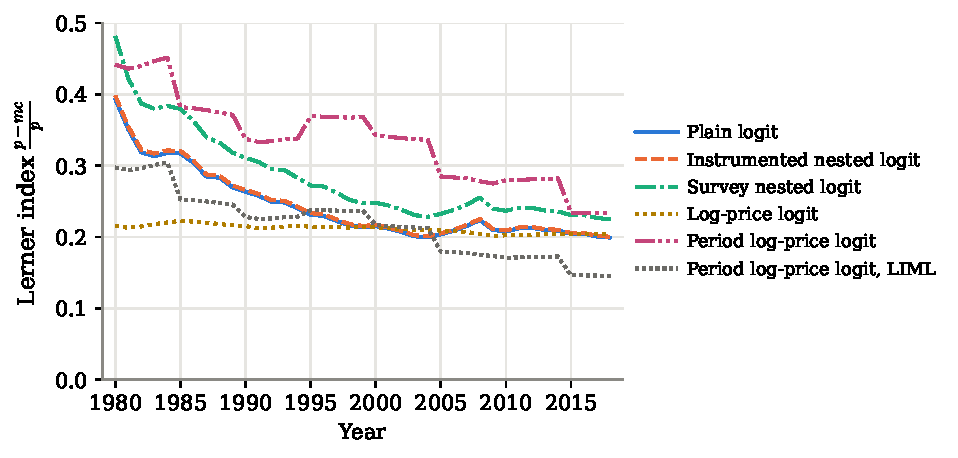
\includegraphics[width=0.95\linewidth]{figures/appC/autos_lerner.pdf}
\caption{Sales-weighted mean Lerner index of new vehicles by year under the six demand models of \cref{tab:C-autos}.
Computed with \texttt{figures/appC/src/autos\_markups.py} from the product data of the replication package of
\citet{GriecoMurryYurukoglu2024}.}
\label{fig:C-autos-lerner}
\end{figure}

\casehead{Part (c)}
Since $L_{jt} = \frac{m_{jt}}{p_{jt}}$, the log Lerner index splits exactly as
\begin{equation}\label{eq:C-lerner-decomp}
  \ln L_{jt} = \ln m_{jt} - \ln p_{jt} = \ln\big(\alpha_\ell m_{jt}\big) - \ln\alpha_\ell - \ln p_{jt} ,
\end{equation}
where $\alpha_\ell$ is the price coefficient that applies in year $t$. It is constant except in the period models of
part (d). We average with the weights $w_{jt}$ and difference between 1980 and 2018. The change in the mean log Lerner index
then splits into the change in the mean log dollar markup and the change in the mean log price. The dollar-markup term
splits again into a scaled markup $\alpha_\ell m_{jt}$ and the coefficient. For the logit with linear price the scaled
markup is $\frac{1}{1 - S_{ft}}$, a function of market structure alone.

\begin{table}[htbp]
\centering
\caption{Decomposition of the change in the mean log Lerner index, 1980 to 2018}
\label{tab:C-autos-decomp}
\footnotesize
\setlength{\tabcolsep}{4pt}
\begin{tabular}{@{}lcccccc@{}}
\toprule
 & Change in & \multicolumn{3}{c}{Dollar markup} & Price & Price share \\
\cmidrule(lr){3-5}
Model & $\overline{\ln L}$ & $\Delta\overline{\ln m}$ & $\Delta\overline{\ln(\alpha_\ell m)}$ & $-\Delta\ln\alpha_\ell$ &
$-\Delta\overline{\ln p}$ & of the fall (\%) \\
\midrule
Plain logit & $-0.694$ & $-0.050$ & $-0.050$ & 0 & $-0.644$ & 93 \\
Instrumented nested logit & $-0.700$ & $-0.056$ & $-0.056$ & 0 & $-0.644$ & 92 \\
Survey nested logit & $-0.765$ & $-0.122$ & $-0.122$ & 0 & $-0.644$ & 84 \\
Log-price logit & $-0.053$ & 0.591 & 0.591 & 0 & $-0.644$ & \\
Period log-price logit & $-0.636$ & 0.008 & 0.591 & $-0.583$ & $-0.644$ & 101 \\
Period log-price logit, LIML & $-0.710$ & $-0.067$ & 0.591 & $-0.658$ & $-0.644$ & 91 \\
\bottomrule
\end{tabular}

\vspace{3pt}
\begin{minipage}{0.97\textwidth}
\footnotesize Notes: Bars denote sales-weighted means within a year, and $\Delta$ the change from 1980 to 2018. The
first column equals the sum of the second and the fifth, and the second equals the sum of the third and the fourth. The
last column is $\frac{\Delta\overline{\ln p}}{-\Delta\overline{\ln L}}$ in percent, omitted where the index barely falls.
Computed with \texttt{figures/appC/src/autos\_markups.py}.
\end{minipage}
\end{table}

\Cref{tab:C-autos-decomp} shows that the decline in every model with a falling index is a fall relative to price. The
sales-weighted mean log price rose by 0.644. Under the plain logit the mean log Lerner index fell by 0.694, so rising
prices account for 93 percent of the fall. The dollar markup fell only 0.050 log points, because firm shares fell and
$\frac{1}{1 - S_{ft}}$ fell with them. The survey nested logit puts more weight on market structure, for a reason we
return to in part (d), but rising prices still account for 84 percent.

\casehead{Part (d)}
The \emph{log-price logit} replaces $\alpha p_{jt}$ by $\alpha\ln p_{jt}$. With the same instrument and controls,
$\hat\alpha = 5.109$ (1.687), and the first-stage $F$ statistic for $\ln p_{jt}$ is 25.1. By
\cref{prop:C-logit-lerner}(ii) the Lerner index stays near $\frac{1}{\hat\alpha} = 0.196$, and indeed it moves only from
0.216 to 0.204. The dollar markup now rises 81 percent, in step with prices. The decomposition shows the mechanism.
By \eqref{eq:C-logprice-markup} the scaled markup $\alpha m_{jt}$ is nearly proportional to price, so its mean log
rises by 0.591 and cancels most of the price term.

Neither functional form is innocuous, and the data can discriminate between them if the price coefficient may change
over time. The \emph{period log-price logit} gives each five-year period $\ell$ its own coefficient $\alpha_\ell$ on
$\ln p_{jt}$. The dollar price sensitivity, the utility lost per dollar, is then $\frac{\alpha_\ell}{p_{jt}}$. If
$\alpha_\ell$ rises in proportion to prices, dollar sensitivity is constant, as in the linear model. If $\alpha_\ell$ is
constant, we are back in the log-price model. Eight coefficients need eight excluded instruments at least. We interact
the exchange rate with period indicators and add assembly-country indicators interacted with period indicators, for
104 excluded instruments, with type-specific linear trends. The added instruments are valid if, within a make,
changes in unobserved quality across periods are unrelated to the assembly country. \citet[fn.~10]{GriecoMurryYurukoglu2024}
strengthen their first stage in the same way when they let the price coefficient vary over time.

\begin{table}[htbp]
\centering
\caption{Period-specific coefficients on log price}
\label{tab:C-autos-periods}
\footnotesize
\begin{tabular}{@{}lccccc@{}}
\toprule
 & \multicolumn{3}{c}{All 104 instruments} & \multicolumn{2}{c}{Exchange rate by period only} \\
\cmidrule(lr){2-4}\cmidrule(lr){5-6}
Period & 2SLS & LIML & OLS & 2SLS & Conditional $F$ \\
\midrule
1980--84 & 2.496 (0.506) & 3.703 & 1.521 & 1.679 (1.782) & 10.8 \\
1985--89 & 2.977 (0.441) & 4.502 & 1.233 & 7.251 (5.634) & 1.9 \\
1990--94 & 3.259 (0.558) & 4.818 & 1.413 & 5.343 (2.399) & 12.6 \\
1995--99 & 2.968 (0.607) & 4.609 & 1.405 & 4.996 (1.802) & 40.5 \\
2000--04 & 3.187 (0.548) & 5.037 & 1.526 & 3.459 (1.229) & 38.5 \\
2005--09 & 3.751 (0.539) & 5.951 & 1.944 & 4.994 (2.227) & 8.1 \\
2010--14 & 3.698 (0.662) & 6.040 & 2.333 & 6.329 (2.478) & 11.1 \\
2015--18 & 4.472 (0.653) & 7.148 & 2.461 & 5.223 (2.581) & 13.6 \\
\bottomrule
\end{tabular}

\vspace{3pt}
\begin{minipage}{0.97\textwidth}
\footnotesize Notes: Entries are $\hat\alpha_\ell$, the negative of the coefficient on $\ln p_{jt}$ in period $\ell$.
The first three columns use the exchange rate by period and assembly-country indicators by period as instruments. The
last two use the eight exchange-rate interactions only. All specifications include the controls of part (a) and
type-specific linear trends. Standard errors clustered by make. Conditional $F$ statistics follow
\citet{SandersonWindmeijer2016}. Computed with \texttt{figures/appC/src/autos\_markups.py}.
\end{minipage}
\end{table}

\Cref{tab:C-autos-periods} reports the coefficients. The 2SLS estimate of $\alpha_\ell$ rises from 2.50 in 1980--84 to
4.47 in 2015--18, an increase of 0.58 log points. Mean log price rose by 0.64, so dollar price sensitivity fell by only
0.06 log points. The dollar markup is then nearly flat (\$7,758 to \$7,851), and the Lerner index falls by 47 percent,
from 0.442 to 0.233. Once the coefficient may follow prices, the data choose a path close to the linear model. Two
caveats apply. With the exchange rate alone the period coefficients are imprecise, and the conditional $F$ statistic
falls to 1.9 in 1985--89, so the path rests on the assembly-country exclusions. With 104 instruments, 2SLS is also
biased toward OLS \citep{Bekker1994}. The OLS coefficients are much smaller, and the limited-information maximum
likelihood (LIML) estimates, which are less sensitive to many instruments, are 48 to 60 percent larger than 2SLS at the
two ends. LIML implies a rise of 0.66 log points in $\alpha_\ell$, lower Lerner indices at every date, and a fall of 51
percent.

The \emph{survey nested logit} replaces the weak instruments for $\sigma$ with information on substitution. A
second-choice survey reports, for buyers of each model, the model they considered most seriously. We treat it as the
model they would have bought had their first choice been unavailable. Its model
counterpart is the effect of removing the first choice from the choice set, a moment that \citet{BerryLevinsohnPakes2004}
introduced into demand estimation.

\begin{lemma}[Removing a model in the nested logit]\label{lem:C-nl-removal}
Suppose model $j$ in nest $g$ is removed and all mean utilities stay fixed. The remaining shares become
\begin{equation}\label{eq:C-nl-removal}
  s'_k = \frac{s_k(1 - s_{j\mid g})^{-\sigma}}{R_j} \ \text{ for } k \in g , \qquad
  s'_k = \frac{s_k}{R_j} \ \text{ otherwise} , \qquad
  R_j = 1 - s_g\big[1 - (1 - s_{j\mid g})^{1 - \sigma}\big] .
\end{equation}
\end{lemma}

\begin{proof}
Removing $j$ multiplies the inclusive sum of nest $g$ by $1 - s_{j\mid g}$, since
$s_{j\mid g} = \frac{e^{\frac{\delta_j}{1 - \sigma}}}{D_g}$, and leaves the other inclusive sums unchanged. The common
denominator $1 + \sum_hD_h^{1 - \sigma}$ is therefore multiplied by
$1 - s_g + s_g(1 - s_{j\mid g})^{1 - \sigma} = R_j$. A model $k \in g$ also has $D_g^{-\sigma}$ in its numerator, which is
multiplied by $(1 - s_{j\mid g})^{-\sigma}$. Substituting in \eqref{eq:C-nl-shares} gives \eqref{eq:C-nl-removal}.
\end{proof}

The survey records only second choices among new vehicles. The model probability that a buyer of $j$ names a second
choice of the same type is therefore
\begin{equation}\label{eq:C-sc-prob}
  \varphi_j(\sigma) = \frac{\sum_{k \in g, k \ne j}(s'_k - s_k)}{\sum_{k \ne j}(s'_k - s_k)} ,
\end{equation}
with both sums over inside models. At $\sigma = 0$ every remaining model gains in proportion to its share, so
$\varphi_j(0) = \frac{s_g - s_j}{1 - s_0 - s_j}$, the IIA answer. Larger $\sigma$ tilts the gains toward the nest. We choose
$\sigma$ so that the average of $\varphi_j(\sigma)$ over surveyed buyers, weighted by the number of respondents whose first
choice is $j$, equals the observed fraction of same-type second choices. That fraction is 84.6 percent. The plain logit
implies 38.2 percent and the instrumented nested logit 46.0 percent. Matching gives $\hat\sigma = 0.524$, with a
bootstrap standard error of 0.002 over the package's 500 resamples of the survey counts. Fitting each survey year
separately gives 0.478 for 1991, 0.567 for 1999, 0.519 for 2005 and 0.532 for 2015. The spread across years is much
larger than the bootstrap standard error, so that standard error understates the uncertainty about a common $\sigma$.

With $\sigma$ fixed at $\hat\sigma$, we move $\hat\sigma\ln s_{j\mid g,t}$ to the left side of \eqref{eq:C-nl-reg} and
estimate $\alpha$ by 2SLS with the exchange rate. Because 2SLS is linear in the dependent variable, the estimate is
$\hat\alpha(\sigma) = 1.696 - 1.795\,\sigma$, where 1.795 is minus the 2SLS coefficient on price in a regression of
$\ln s_{j\mid g,t}$. At $\hat\sigma = 0.524$ this gives $\hat\alpha = 0.755$. Its two-step standard error, which adds
$1.795^2$ times the variance of $\hat\sigma$, is 0.302. The model implies higher Lerner indices, 0.481 in 1980 and
0.225 in 2018, and a fall in the dollar markup of 12.3 percent. Market structure explains the larger fall. Nested logit markups depend on the firm's share within each type. The sales-weighted mean
within-type share of a model's firm fell from 0.280 to 0.137 as the number of models per type grew.

\casehead{Part (e)}
Four lessons emerge. First, simple models on the package data reproduce the broad decline. The plain logit and the
nested logits all put the 2018 index at about half its 1980 value. The full model of \citet{GriecoMurryYurukoglu2024}
gives a sales-weighted mean Lerner index of 0.42 in 1980 and 0.22 in 2018 (Section~5.4 and Table~VII), a ratio of
0.52. Our plain logit gives 0.393 and 0.199, a ratio of 0.506. We describe their model after the four lessons.

Second, the decline is a fall in markups relative to price. In every model except the log-price logit, the mean dollar
markup changes by between $-12.3$ and $+1.2$ percent, while the mean real price nearly doubles. Under linear price this
stability is built in, since by \cref{prop:C-logit-lerner} the dollar markup depends only on $\alpha$ and on shares. A
falling Lerner index with stable dollar markups is what rising quality and marginal cost produce. It does not mean that
firms earn less per vehicle.

Third, the functional form of price decides the trend once the price coefficient is held fixed. Linear price builds in
a Lerner index proportional to $\frac{1}{p}$, and log price builds in a flat one. \citet{GriecoMurryYurukoglu2024}
report a much smaller decline in their own log-price specification, from 0.32 to 0.27 (Section~5.4). With log price
and a separate coefficient for each five-year period, their path looks very similar to their baseline (Figure~VIb).
When the coefficient on log price may change over time, our estimates also move it almost in proportion to prices,
which supports the linear form. That conclusion rests on 104 instruments and on exclusions by assembly country. A cost shifter
that varies more across periods, such as wages in the assembly countries, would test it directly.

Fourth, the substitution parameters matter for levels more than for trends. The survey nested logit raises the Lerner
index by about 0.09 in 1980 and 0.03 in 2018 relative to the plain logit. Aggregate data alone cannot pin down $\sigma$
(\cref{tab:C-autos-nl}), and the second-choice survey can. This is the same lesson as in \cref{sec:C-rc-est}, where the
logit understated diversion among inside goods.

The full model of \citet{GriecoMurryYurukoglu2024} differs from ours in its demand system, its data and its estimator.
Their demand is a random coefficients logit in the tradition of \citet{BerryLevinsohnPakes1995}. In our notation,
household $i$ in year $t$ obtains
\begin{equation}\label{eq:C-gmy-utility}
  u_{ijt} = x_{jt}\beta_{it} - \alpha_{it}p_{jt} + \xi_{jt} + \epsilon_{ijt} , \qquad u_{i0t} = \gamma_t + \epsilon_{i0t} ,
\end{equation}
from model $j$ and from the outside good (their eq.~1). The value $\gamma_t$ of not buying a new vehicle changes from
year to year. Let $D_{it}$ be the vector of household demographics, drawn from the CPS. It has nothing to do with the
inclusive sums $D_{gt}$ of part (a). The coefficients are
\begin{equation}\label{eq:C-gmy-coef}
  \alpha_{it} = \alpha + \pi^\top D_{it} , \qquad \beta_{ikt} = \beta_k + \Pi_kD_{it} + \Sigma_{kk}\nu_{ik} ,
\end{equation}
where $\Pi_k$ is the $k$-th row of $\Pi$ and the $\nu_{ik}$ are independent standard normal draws (eqs.~3--4). The
parameters are fixed over time, but the distribution of tastes moves as demographics change. In our sign convention the
mean price coefficient is $\alpha = 3.112$ (1.124) per \$10,000 (Table~IV). Price sensitivity varies with income, its
square and age. Family size shifts the tastes for vans and for footprint, and rural households value trucks more. Eleven
characteristics carry random coefficients. The two largest are on vehicle types, 6.309 for trucks and 5.538 for vans.
The SUV coefficient of 3.617 is close to the largest remaining one, 3.798 for electric vehicles. The type coefficients
play the role of our nests, since a household with a strong taste for trucks substitutes mainly among trucks.

The year effects mix two objects. GMY write $\xi_{jt} = \tau_t + \tilde\xi_{jt}$, where $\tau_t$ is the mean
unobserved quality of the models of year $t$ relative to the base year. Shares identify only the difference
$\tau_t - \gamma_t$. Following \citet{PakesBerryLevinsohn1993}, GMY assume that unobserved quality does not change on
average for models that continue from $t - 1$ to $t$ without a redesign. With $\mathcal{C}_t$ the set of such models,
\begin{equation}\label{eq:C-gmy-continuing}
  \E\big[\xi_{jt} - \xi_{j,t-1}\big] = \E\big[(\tau_t - \tau_{t-1}) + (\tilde\xi_{jt} - \tilde\xi_{j,t-1})\big] = 0
  \qquad \text{for } j \in \mathcal{C}_t ,
\end{equation}
with the normalization $\tau_0 = 0$ (eq.~2). The condition separates better vehicles from a more attractive outside
option. Mean unobserved quality rises roughly linearly, by about \$25,000 over the period (Section~5.2).

Estimation has three steps (Section~5). The first step chooses the demographic interactions, the random coefficients
and the mean utilities by GMM. It matches two kinds of micro moments. The CEX (1980--2005, about 1,014 buyers a year)
and MRI (1992--2018, about 2,005 buyers a year) give moments such as the mean price paid in each income quintile
(Sections~2.3 and~5). The MaritzCX survey gives the correlations between the attributes of first and second choices in the
four survey years. The second step regresses the mean utilities on characteristics, price, make dummies and year
dummies by 2SLS, with the lagged real exchange rate as the excluded instrument. This is the moment condition of our part
(a). The third step splits the year effects into $\tau_t$ and $\gamma_t$ with \eqref{eq:C-gmy-continuing}. Standard
errors come from 500 bootstrap samples of the micro data, with a nested parametric bootstrap, clustered by make, in the
second step.

Each source of variation has a clear role. The real exchange rate is the price level of the assembly country relative
to the United States, taken from the Penn World Table and lagged one year (Section~2.2). It moves with local wages and
with the nominal exchange rate, and both shift the dollar cost of the vehicles made there. It identifies the price
coefficient. The second choices identify the random coefficients. The correlation between the truck indicators of first
and second choices is 0.843 in the data and 0.798 in the full model (Table~VI). A model with the demographic
interactions alone gives $-0.013$, and the logit gives $-0.024$. Observed heterogeneity alone cannot produce the
substitution within types that the survey records. Our survey nested logit in part (d) rests on the same evidence.

The full model gives a share-weighted mean own-price elasticity of $-5.06$ over the sample (Section~5.1). The market
elasticity is $-1.07$ in 1985 and $-1.29$ in 2015 (Table~V). The median Lerner index falls from 0.325 to 0.185
(Figure~VIa). The decline survives a linear trend in the price coefficient, a separate coefficient for each five-year
period and separate estimation on three subperiods (Figure~VIb).

GMY explain the decline much as part (c) does. Single-product markups follow nearly the same path as multi-product ones
(Figure~VIIIa). The single-product rule $L_{jt} = -\frac{s_{jt}}{p_{jt}}\big(\frac{\partial s_{jt}}{\partial
p_{jt}}\big)^{-1}$ of their eq.~(7) therefore guides the reading. From 1980 to 1999, mean shares and mean own-price
derivatives stay flat while mean prices rise, so the index falls. Counterfactuals then isolate the primitive forces
(Section~5.4.1). Removing the growth of foreign brands from the ownership structure, or holding the number of products
at its 1980 level, does not remove the decline. Mapping each year's characteristics onto their 1980 distribution keeps
marginal costs flat and substantially reduces the fall (Figure~IX). In their reading, better vehicles raised marginal
costs, which were passed through to prices less than fully.

GMY maintain Nash-Bertrand pricing and ask how much collusion would be needed to undo the decline (Section~5.5).
Simulated cartels in 2018 answer the question in Table~VII. A cartel of GM, Ford and Toyota raises the mean Lerner index
only to 0.26. Only a cartel of the six largest parent companies, at 0.46, exceeds the 1980 value of 0.42. The
Herfindahl index meanwhile fell from 2,661 to 1,132 points. Beyond markups, the consumers' share of efficient surplus
rose from 0.62 to 0.82, and consumer surplus per household rose by about \$8,000 (Section~1). GMY define efficient
surplus as consumer surplus plus producer surplus plus deadweight loss, the surplus at prices equal to marginal costs.
Our simple models agree with the full model on the main mechanism. Prices rose against stable dollar markups. GMY
report no dollar markups. By their eq.~(7), however, flat mean shares and own-price derivatives imply flat
single-product dollar markups from 1980 to 1999 (Section~5.4.1 and Figure~VIII). What the full model adds is the separation of
quality from the outside option and a measure of welfare.

The exercise has clear limits. Prices are list prices, so changes in discounts and rebates over time pass into the
estimated markups. The market size of one vehicle per 2.5 households is a convention, and the outside share moves with
it. Demand is static, with no used-car market or replacement timing, and the nests are chosen a priori. The exchange
rate may violate the exclusion if currency movements coincide with changes in a make's unobserved quality. The
comparison with production-function estimates is also less direct than it looks. The demand-side Lerner index measures
price over marginal cost for new vehicles, while production-function markups use firm-level revenue and variable
input costs (\cref{sec:01-rising-markups}). \citet[Section~5.6]{GriecoMurryYurukoglu2024} make this comparison for the
auto industry. Both the level and the trend of their ratio of price to marginal cost differ from the production-function
series, although both are fairly flat after 1995. What the exercise contributes is a diagnosis. It shows which parts of a
measured trend in markups come from the data, which from the functional form, and which from the estimated
substitution patterns.

\subsection{Computational notes}

The script \texttt{autos\_markups.py} reads the package files \texttt{data\_blp.csv}, \texttt{secondChoiceOut.mat}
and \texttt{secondChoice\_bootstrap.mat}, and it runs in about three minutes.
\begin{enumerate}
  \item Build shares with $M_t$ equal to households divided by 2.5, prices in \$10,000, nests from the type indicators,
  and within-type shares and counts by year and type.
  \item Code 2SLS, the clustered sandwich, first-stage and conditional $F$ statistics and LIML with numpy. Run the
  logit, the nested logit grid and the log-price models.
  \item Fit $\sigma$ to the second-choice counts with a bracketing root finder on $[0, 0.995]$, using
  \eqref{eq:C-nl-removal} and \eqref{eq:C-sc-prob}, and repeat for each bootstrap sample of counts.
  \item For each model and year, form $\Delta_t$ from \eqref{eq:C-nl-deriv} or its log-price analogue and solve
  \eqref{eq:C-autos-markup} with the parent-company ownership matrix.
  \item Check the share inversion, the removal formula against brute-force removal, the derivatives against finite
  differences and the logit markups against \cref{prop:C-logit-lerner}.
\end{enumerate}
